\documentclass[
  %fleqn,     das ist für die zentrierung
	parskip=half,
	captions=tableheading,
  titlepage=firstiscover, 		%************************************************** by Rk
	bibliography=totoc		%*************************************by Rk
	]{scrartcl}			
% \usepackage{etex}
% \reserveinserts{28}

%Das ist für die Kopfzeile
\usepackage[headsepline]{scrlayer-scrpage}
\pagestyle{scrheadings}
\clearpairofpagestyles
\ofoot{\pagemark}
\ohead{\headmark}
\automark{section}

% Warnung, falls nochmal kompiliert werden muss		%*************************************by Rk
\usepackage[aux]{rerunfilecheck}

% unverzichtbare Mathe-Befehle
\usepackage{amsmath}
% viele Mathe-Symbole
\usepackage{amssymb}
% Erweiterungen für amsmath
\usepackage{mathtools}
\usepackage{upgreek}
% Fonteinstellungen
\usepackage{fontspec}				%************************************************** by Rk
% Latin Modern Fonts werden automatisch geladen
% Latin Modern Fonts werden automatisch geladen
% Alternativ zum Beispiel:
%\setromanfont{Libertinus Serif}
%\setsansfont{Libertinus Sans}
%\setmonofont{Libertinus Mono}

\usepackage{polyglossia}
\usepackage[				%************************************************** by Rk
	backend=biber,
]{biblatex}  	
%Quellendatenbank	
\setmainlanguage{german}			
\addbibresource{lit.bib}		%************************************************** by Rk


\usepackage{expl3}
\usepackage{xparse}

\usepackage{physics}

\usepackage[unicode, german]{hyperref}
\usepackage[autostyle]{csquotes}
\usepackage[
  math-style=ISO,    % ┐
  bold-style=ISO,    % │
  sans-style=italic, % │ ISO-Standard folgen
  nabla=upright,     % │
  partial=upright,   % ┘
  warnings-off={           % ┐
    mathtools-colon,       % │ unnötige Warnungen ausschalten
    mathtools-overbracket, % │
  },                       % ┘
]{unicode-math}

% traditionelle Fonts für Mathematik
\setmathfont{Latin Modern Math}
% Alternativ zum Beispiel:
%\setmathfont{Libertinus Math}

\setmathfont{XITS Math}[range={scr, bfscr}]
\setmathfont{XITS Math}[range={cal, bfcal}, StylisticSet=1]

% Zahlen und Einheiten
\usepackage[
  locale=DE,                 % deutsche Einstellungen
  separate-uncertainty=true, % immer Fehler mit \pm
  per-mode=symbol-or-fraction,       % ^-1 für inverse Einheiten
  % output-decimal-marker=.,   % . statt , für Dezimalzahlen
]{siunitx}

% chemische Formeln
\usepackage[
  version=4,
  math-greek=default, % ┐ mit unicode-math zusammenarbeiten
  text-greek=default, % ┘
]{mhchem}

% Wenn man andere Schriftarten gesetzt hat,
% sollte man das Seiten-Layout neu berechnen lassen
\recalctypearea{}				%************************************************** by Rk


% richtige Anführungszeichen 
\usepackage[autostyle]{csquotes}

% schöne Brüche im Text
\usepackage{xfrac}

% Grafiken können eingebunden werden
\usepackage{graphicx}
% größere Variation von Dateinamen möglich
% \usepackage{grffile}
\usepackage{scrhack}

% Verbesserungen am Schriftbild
\usepackage{microtype}

% Standardplatzierung für Floats einstellen
\usepackage{float}
\usepackage[section, below]{placeins}
% \usepackage[..]{caption}
\floatplacement{figure}{htbp}
\floatplacement{table}{htbp}

\usepackage{booktabs}
\usepackage{subcaption}
% \usepackage{subfig}
\author{%
  Raphael Rico Kaiser\\%
  \href{raphael.kaiser@tu-dortmund.de}{raphael.kaiser@tu-dortmund.de}%
  \texorpdfstring{\and}{,}%
  Hendrik Trojan\\%
  \href{hendrik.trojan@tu-dortmund.de}{hendrik.trojan@tu-dortmund.de}%
}

\publishers{TU Dortmund - Fakultät Physik}
\usepackage{romannum}
\AtBeginDocument{\pagenumbering{arabic}}

\NewDocumentCommand \e {}
{
  \symup{e}
}

\NewDocumentCommand \const {}
{
  \text{const.}
}

\NewDocumentCommand \fig {mmm}
{
\begin{figure}
    \centering 
    \includegraphics[width=9cm]{#1}
    \caption{#3}
    \label{#2}
   \end{figure}
\nocite{*}
}

\usepackage{romannum}
\usepackage{listings}
\lstset{numbers=left, numberstyle=\tiny, numbersep=5pt}
\lstset{language=Perl}
\AtBeginDocument{\pagenumbering{arabic}}

\title{
\includegraphics[scale=0.8]{../logo.jpg} \\ \vspace*{1cm} VXX \\ - xxx -}

%\title{test}
\date{Durchführung: xx.xx.2021, Abgabe: xx.xx.2021}

\begin{document}

\maketitle

\tableofcontents
\newpage

\section{Ziel}
Das Ziel dieses Versuchs ist es die Funktionsweise eines Sagnac-Interferometers zu verstehen. Der Strahlengang soll justiert werden und es sollen der Kontrast des Interferometers, der Brechungsindex von Glas sowie der Brechungsindex von Luft bestimmt werden.
%Vorteile von Sagnac hier erwähnen?

\section{Theorie}
%Quellen einfügen
%Polarisationswinkel und Winkel Glasplatten umbenennen!!!

\subsection{Interferenz und Kohärenz}
%Interferenz:
Überlagern sich zwei Wellen, kann es zu Interferenz kommen. Eine Bedingung dafür ist, dass die Wellen die selbe Wellenlänge besitzen.
%Superpositionsprinzip:
\dots
%konstruktive und destruktive Interferenz:
\dots
Die Interferenz ist stabil, wenn die Wellen kohärent sind.

%Kohärenz:
Der Begriff der Kohärenz beschreibt die Tatsache, dass die Wellen untereinander eine feste Phasenbeziehung haben.
%Kohärenzzeit:
Die Wellenlänge der sich überlagernden Wellen ist während der Kohärenzzeit gleich. Diese ist die Zeit, in der sich eine Welle nicht ändert.
Laserlicht hat eine hohe Kohärenzzeit, weswegen es in optischen Versuchen bevorzugt wird.
%Zeitliche Kohärenz:
\dots
%Räumliche Kohärenz:
\dots
%Kohärenzgrad:
Der Kohärenzgrad beschreibt die Interferenzfähigkeit zweier Wellen.

\subsection{Polarisation}
%linear, elliptisch, zirkular:
Die Polarisation einer Transversalwelle, z.B. Licht, beschreibt ihre Schwingungsrichtung. Es wird zwischen linearer, elliptischer und zirkularer Polarisation unterschieden. Bei den beiden letzteren dreht sich die Richtung der Schwingung um die Ausbreitungsrichtung der Welle. Bei linearer Polarisation ist die Richtung der Schwingung konstant. Diese wird als Winkel in Bezug auf eine bestimmte Ebene oder als Anteil der parallelen und senkrechten Komponenten angegeben.

%p- und s-polarisiert:
Trifft linear polarisiertes Licht auf eine Grenzfläche, wird der Anteil, der parallel zu der Spiegelebene polarisiert ist (p-polarisiert), transmittiert und der senkrecht zu dieser Ebene polarisierte Anteil (s-polarisiert) wird reflektiert. Das ist schematisch in \autoref{fig:sppolarisation} zu sehen.

%Bezug zu Interferenz:
Damit zwei Wellen nun interferieren können, müssen sie gleich polarisiert sein, damit sich die elektrischen Felder aufheben können. Das ist bei p- und s-polarisiertem Licht etwa durch einen Polarisationsfilter umsetzbar.

\begin{figure}
    \centering
    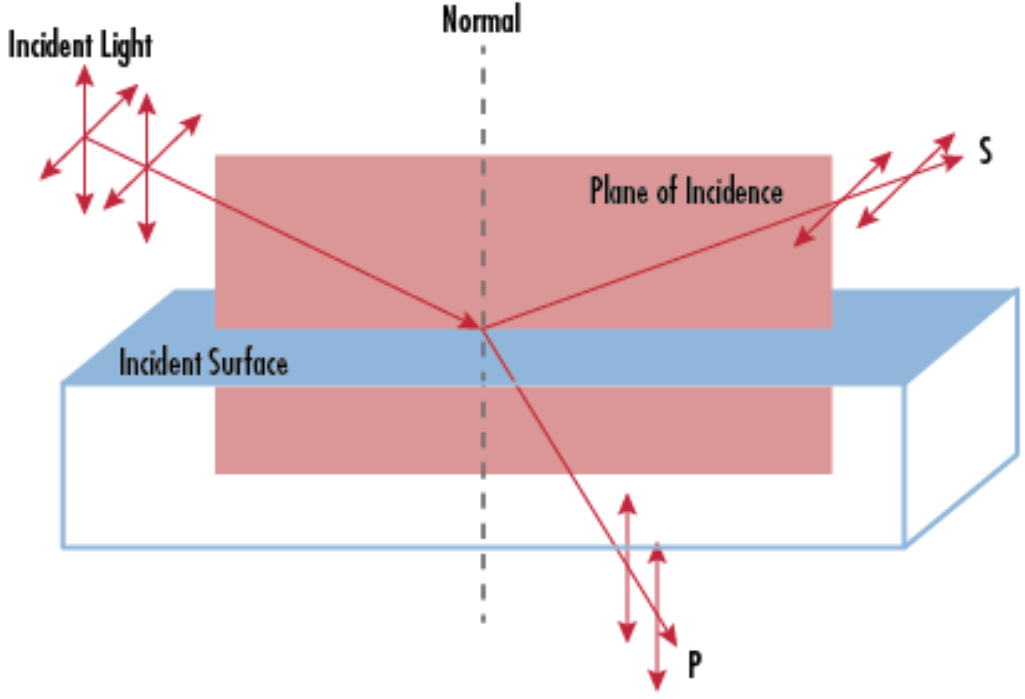
\includegraphics[width=0.6\linewidth]{./figures/s_p_polarisation.png}
    \caption{s- und p-Polarisation. Quelle: https://www.edmundoptics.de/knowledge-center/application-notes/optics/introduction-to-polarization/}
    \label{fig:sppolarisation}
\end{figure}



\subsection{Kontrast eines Interferometers}
Der Kontrast ist ein Maß für die Qualität des Interferenzbildes eines Interferometers. Er ist über die Intensität des Interferenzmaximums und -minimums definiert
\begin{equation}
    K = \frac{I_{max}-I_{min}}{I_{max}+I_{min}} \, .
    \label{eq:kontrast}
\end{equation}
Der Kontrast kann minimal Null sein. Das ist der Fall, wenn ein Interferenzmaximum und -minimum nicht unterscheidbar sind, die Qualität also schlecht ist.
Maximal kann der Kontrast Eins sein. In diesem Fall ist das Minimum perfekt ausgelöscht.

Da der Kontrast über die Intensität definiert ist und diese Abhängig vom Polarisationswinkel ist, kann folgende Proportionalität angegeben werden
\begin{equation*}
    K(\phi) \propto = | 2 \cos{(\phi)} \sin{(\phi)} | = |\sin{(2\phi)}| \, .
\end{equation*}
%Diese folgt aus \autoref{eq:intensitaet}. %noch hinzufügen



\subsection{Brechungsindizes von Luft und Glas}
\textbf{Brechungsindex von Luft}

Um den Brechungsindex eines Mediums zu bestimmen, werden die Strahlen im Interferometer aufgeteilt und geometrisch voneinander getrennt, sodass sie unterschiedliche Medien durchlaufen können. Ein Strahl, der ein Medium durchlaufen hat, ist gegenüber einem Strahl im Vakuum phasenverschoben. Bei Zusammenführung der Strahlen interferieren sie und anhand der Interferenzmaxima kann der Brechungsindex abgeleitet werden. %Minima??

Ein Strahl, der eine evakuierte Kammer der Länge $L$ durchläuft, hat zu einem durch Luft laufenden Strahl eine relative Phasenverschiebung von %bzw: ein mit Gas gefüllter Körper erzeugt diese Phasenverschiebung ?
\begin{equation*}
    \Delta \delta = \frac{2 \pi L}{\lambda_{0}} (n-1) .
\end{equation*}
Dabei ist $\lambda_0$ die Wellenlänge im Vakuum und $n$ der Brechungsindex von Luft.

Die Phasenverschiebung hängt mit der Anzahl der Maxima über folgende Formel zusammen 
\begin{equation*}
    M = \frac{\Delta \delta}{2 \pi} . 
\end{equation*}

Aus diesen Zusammenhängen ergibt sich für den Brechungsindex die Gleichung
\begin{equation}
    n = \frac{M \lambda_0}{L} + 1 \, .
    \label{eq:brechungsindex}
\end{equation}

Aus dem Lorentz-Lorenz Gesetz
%\begin{equation*}
%    \frac{n^2 - 1}{n^2 + 2} = \frac{N \alpha}{3 \epsilon_0}
%\end{equation*}
ergibt sich näherungsweise für den Brechungsindex in Abhängigkeit vom Druck $p$ folgende Gleichung
\begin{equation*}
    n(p) \approx \frac{3 A p}{2 R T} + 1 \,.
    \label{eq:n_p}
\end{equation*}
Dabei ist $A$ die Molreflektivität, $R$ die universelle Gaskonstante und $T$ die Temperatur.
\\


\textbf{Brechungsindex von Glas}

Auch für die Bestimmung des Brechungsindex von Glas sind die Teilstrahlen geometrisch getrennt. Läuft einer der Strahlen durch eine planparallele Platte, entsteht eine relative Phasenverschiebung von
\begin{equation*}
    \Delta \delta = \frac{2 \pi D}{\lambda_0} \left[ \frac{n-1}{2n} \phi^2 + {\mathcal{O}}(\phi^4) \right] \, .
\end{equation*}
In diesem Versuch werden zwei Glasplatten, durch die je ein Teilstrahl läuft, verwendet. Diese sind konstant um $\phi_0 = 20 \degree$ verkippt %stimmt die Zahl?
und werden um den Winkel $\phi$ gedreht.
Die Interferenzmaxima sind gegeben durch
\begin{equation*}
    M = \frac{D}{\lambda_0} \frac{n-1}{2n} \left[ \left( \phi + \frac{\phi_0}{2} \right)^2 - \left( \phi - \frac{\phi_0}{2} \right)^2 \right] \, .
\end{equation*}

Der vom Drehwinkel abhängige Brechungsindex ist dann
\begin{equation}
    n(\phi) = \frac{1}{1-\frac{M \lambda_0}{2 \phi_0 \phi D}} \, .
    \label{eq:n_phi}
\end{equation}
Hier ist \dots



\section{Durchführung}
%Fotos ergänzen
%paar Infos ergänzen

\subsection{Aufbau}
Bei einem Sagnac-Interferometer wird das Licht eines Lasers durch einen sogenannten Polarizing Beam Splitter Cube (PBSC) in zwei Strahlen aufgeteilt, die mittels Spiegeln in entgegengesetzter Richtung im Kreis geführt werden und am PBSC wieder aufeinander treffen. Durch die gegenläufige Richtung der Strahlen wird ein zeitlich besonders stabiles Interferenzbild erzeugt.

Das Licht des hier verwendeten Helium-Neon-Lasers mit einer Wellenlänge von $\lambda = \SI{632.99}{\nano\meter}$ wird mit zwei Spiegeln durch einen linearen Polarisationsfilter in das Interferometer gelenkt.

Der Lichtstrahl trifft zunächst auf den PBSC. Dieser besteht aus zwei Prismen und hat diagonal eine dielektrische Schicht. Dort wird p-polarisiertes Licht transmittiert und s-polarisiertes Licht reflektiert.
Die beiden Strahlen überlappen beim Durchgang durch das Interferometer, werden am PBSC wieder zu einem Strahl vereint und treffen danach entweder durch einen zweiten Polarisationsfilter auf einen Schirm oder durch einen zweiten PBSC auf zwei Photodioden.

Der Aufbau sowie der Strahlengang sind in \autoref{fig:aufbau} zu sehen.
\autoref{fig:fotos} zeigt Fotos des Aufbaus.

\begin{figure}
    \centering
    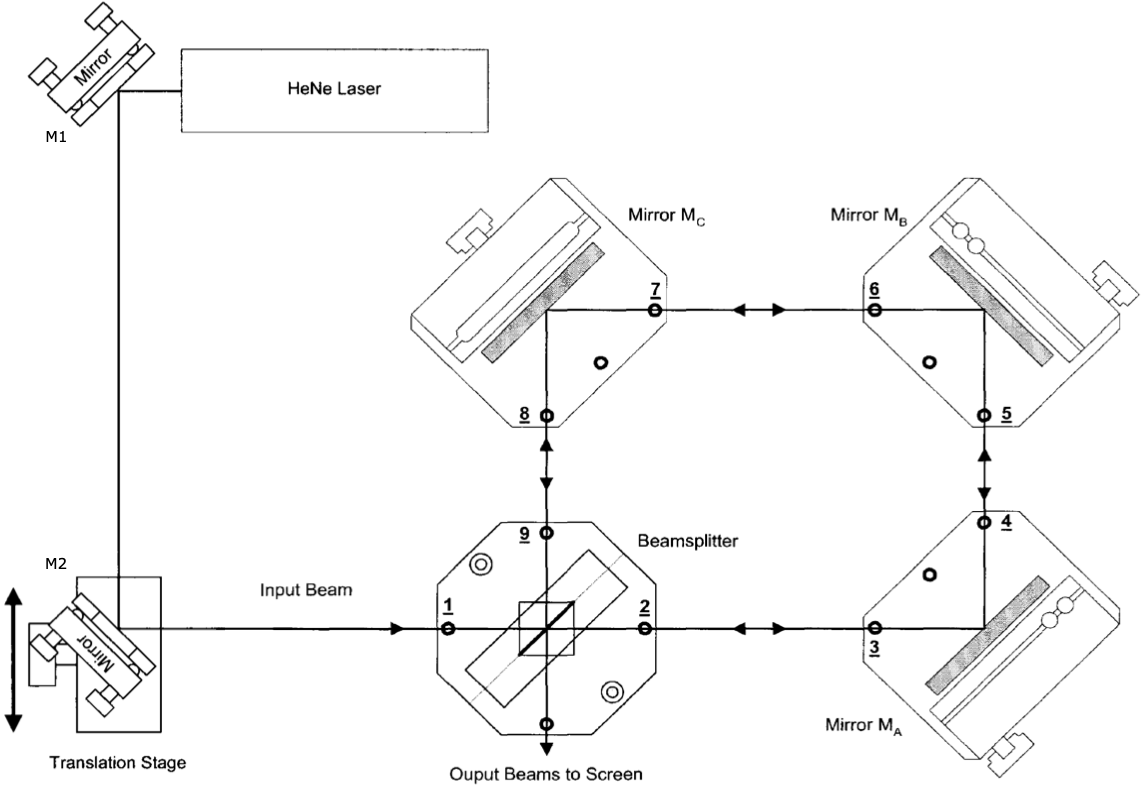
\includegraphics[width=0.7\linewidth]{./figures/aufbau.png}
    \caption{Der Aufbau. \cite{Anleitung}}
    \label{fig:aufbau}
\end{figure}

\begin{figure}
    \centering
    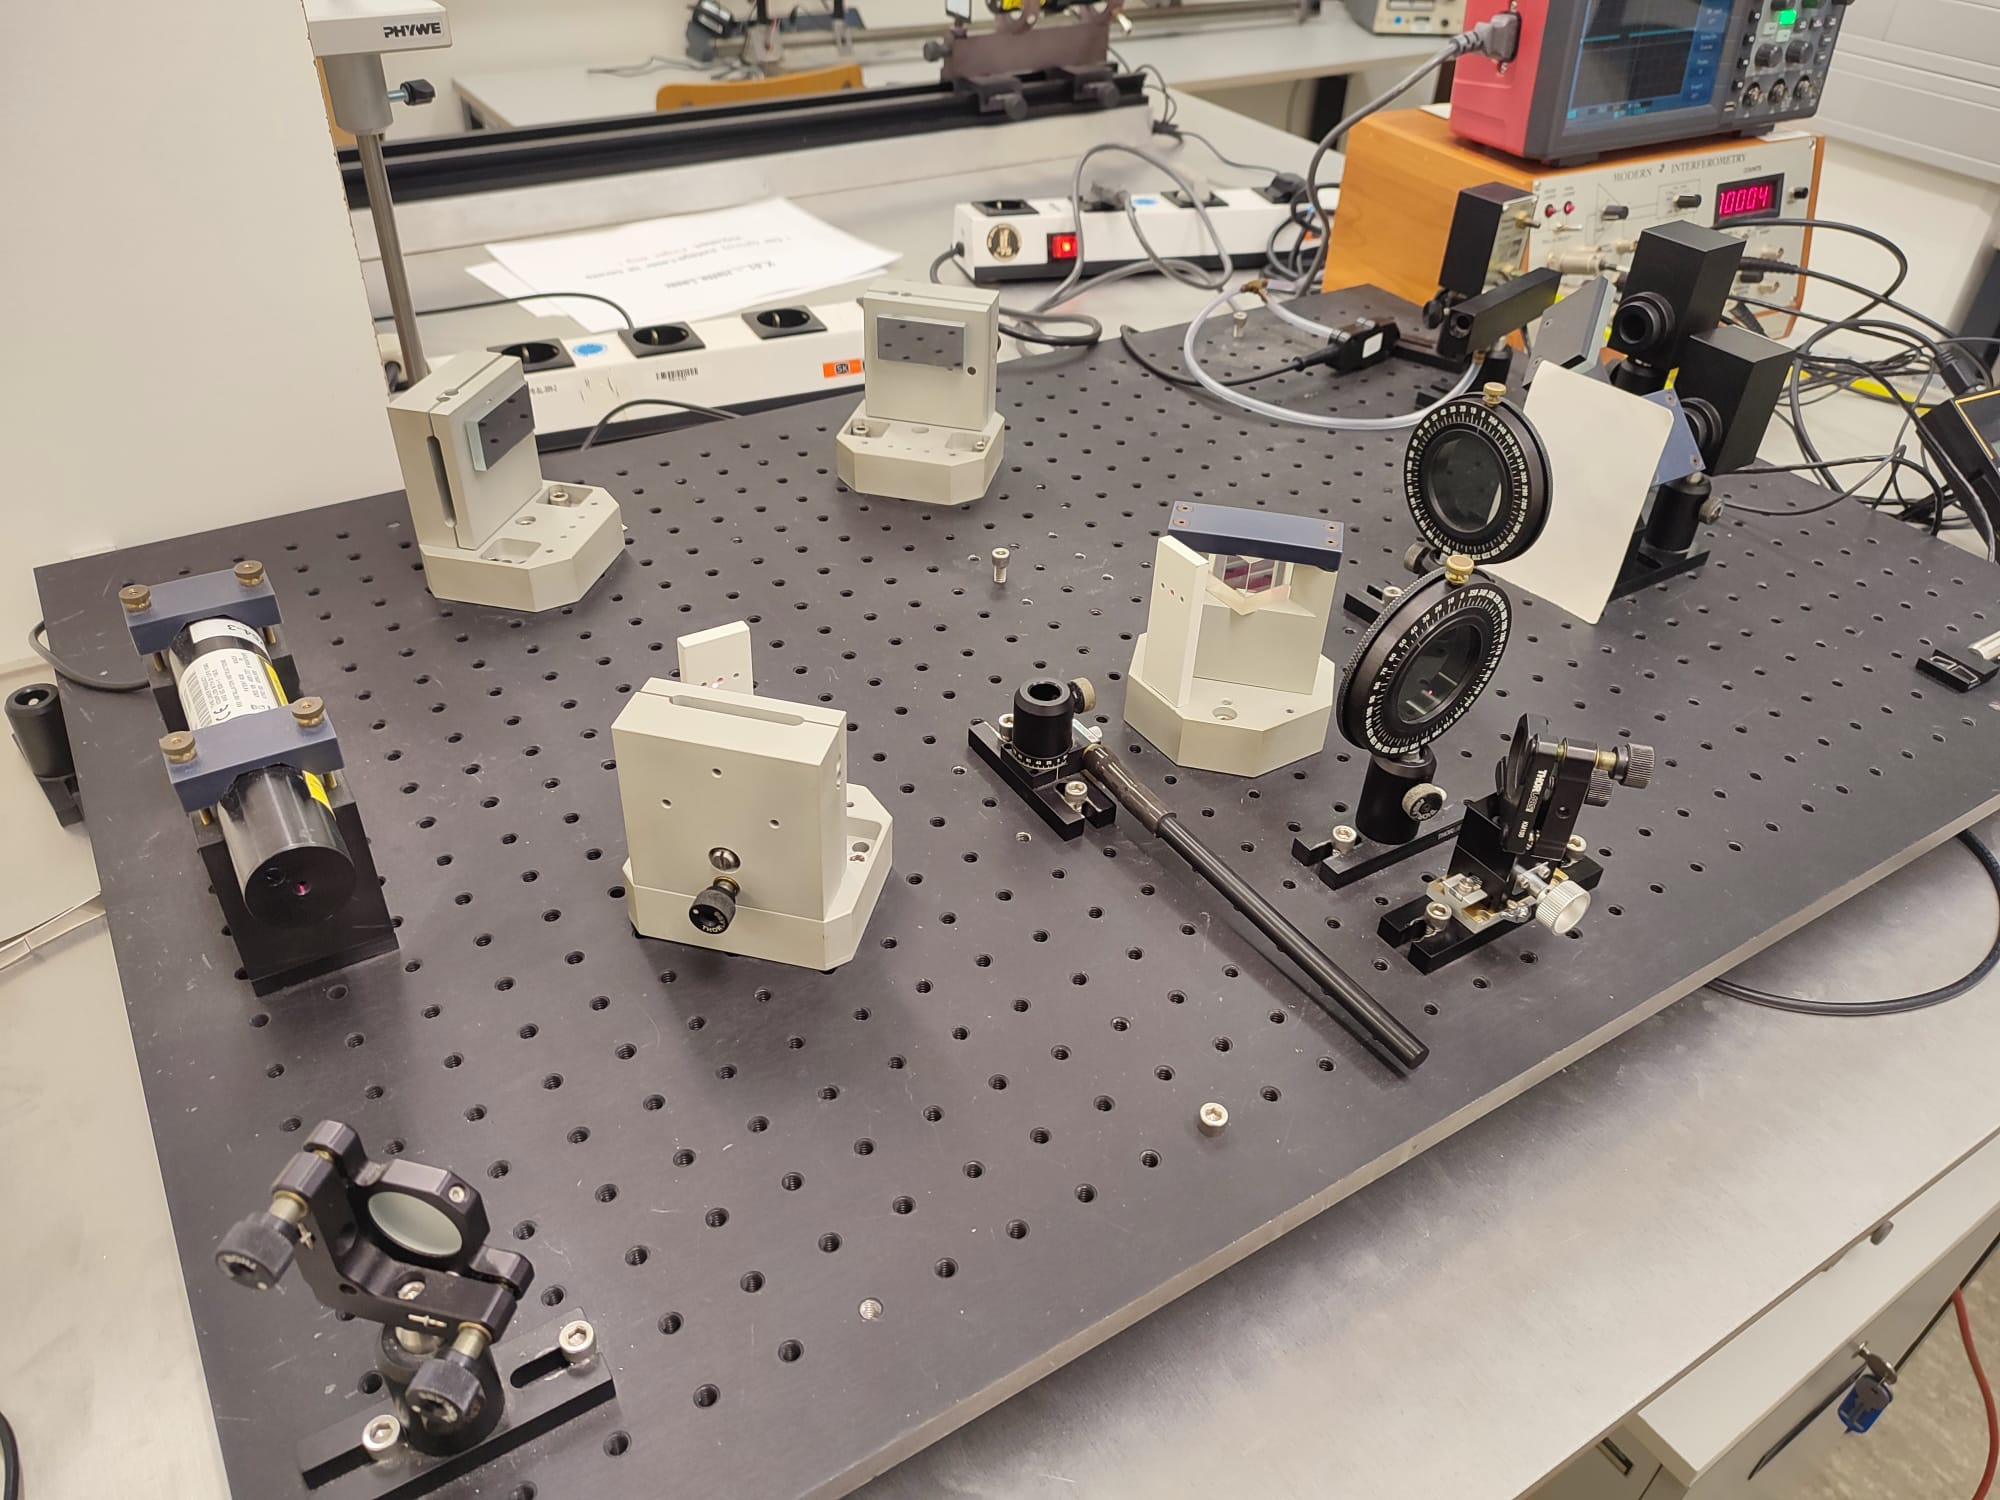
\includegraphics[width=0.7\linewidth]{./figures/aufbau_foto.jpeg}
    \caption{Fotos des Aufbaus.}
    \label{fig:fotos}
\end{figure}

\subsection{Justierung}
Zunächst wird der Strahlengang im Interferometer durch Ausrichtung der Bodenplatten der Spiegel sowie Einstellen der Feinjustierschrauben ausgerichtet. Dazu werden zunächst die Spiegel M1 und M2 abwechselnd so ausgerichtet, dass der vom PBSC transmittierte Strahl (dieser ist p-polarisiert) mittig auf Spiegel $M_A$ fällt. Dazu werden die Justageplatten benutzt und der reflektierte (s-polarisierte) Strahl wird abgeschirmt. Anschließend wird der reflektierte Strahl auf die selbe Weise auf Spiegel $M_C$ ausgerichtet. Die von $M_A$ und $M_C$ kommenden Strahlen, die auf Spiegel $M_B$ treffen sollen, werden ebenfalls mit Hilfe der Justageplatten justiert. Schließlich wird Spiegel $M_B$ ausgerichtet und die Strahlen treffen sich im PBSC.

Damit die nun überlappenden, noch senkrecht zueinander polarisierten Strahlen interferieren können, wird ein Polarisationsfilter hinter dem Interferometer eingesetzt. Dieser wird auf $45 \degree$ gestellt, sodass die Strahlen in derselben Polarisationsebene liegen und ein Muster aus Interferenzstreifen entsteht.% (siehe \autoref{fig:streifen}).

%\begin{figure}
%    \centering
%    \subfigure[Streifen.]{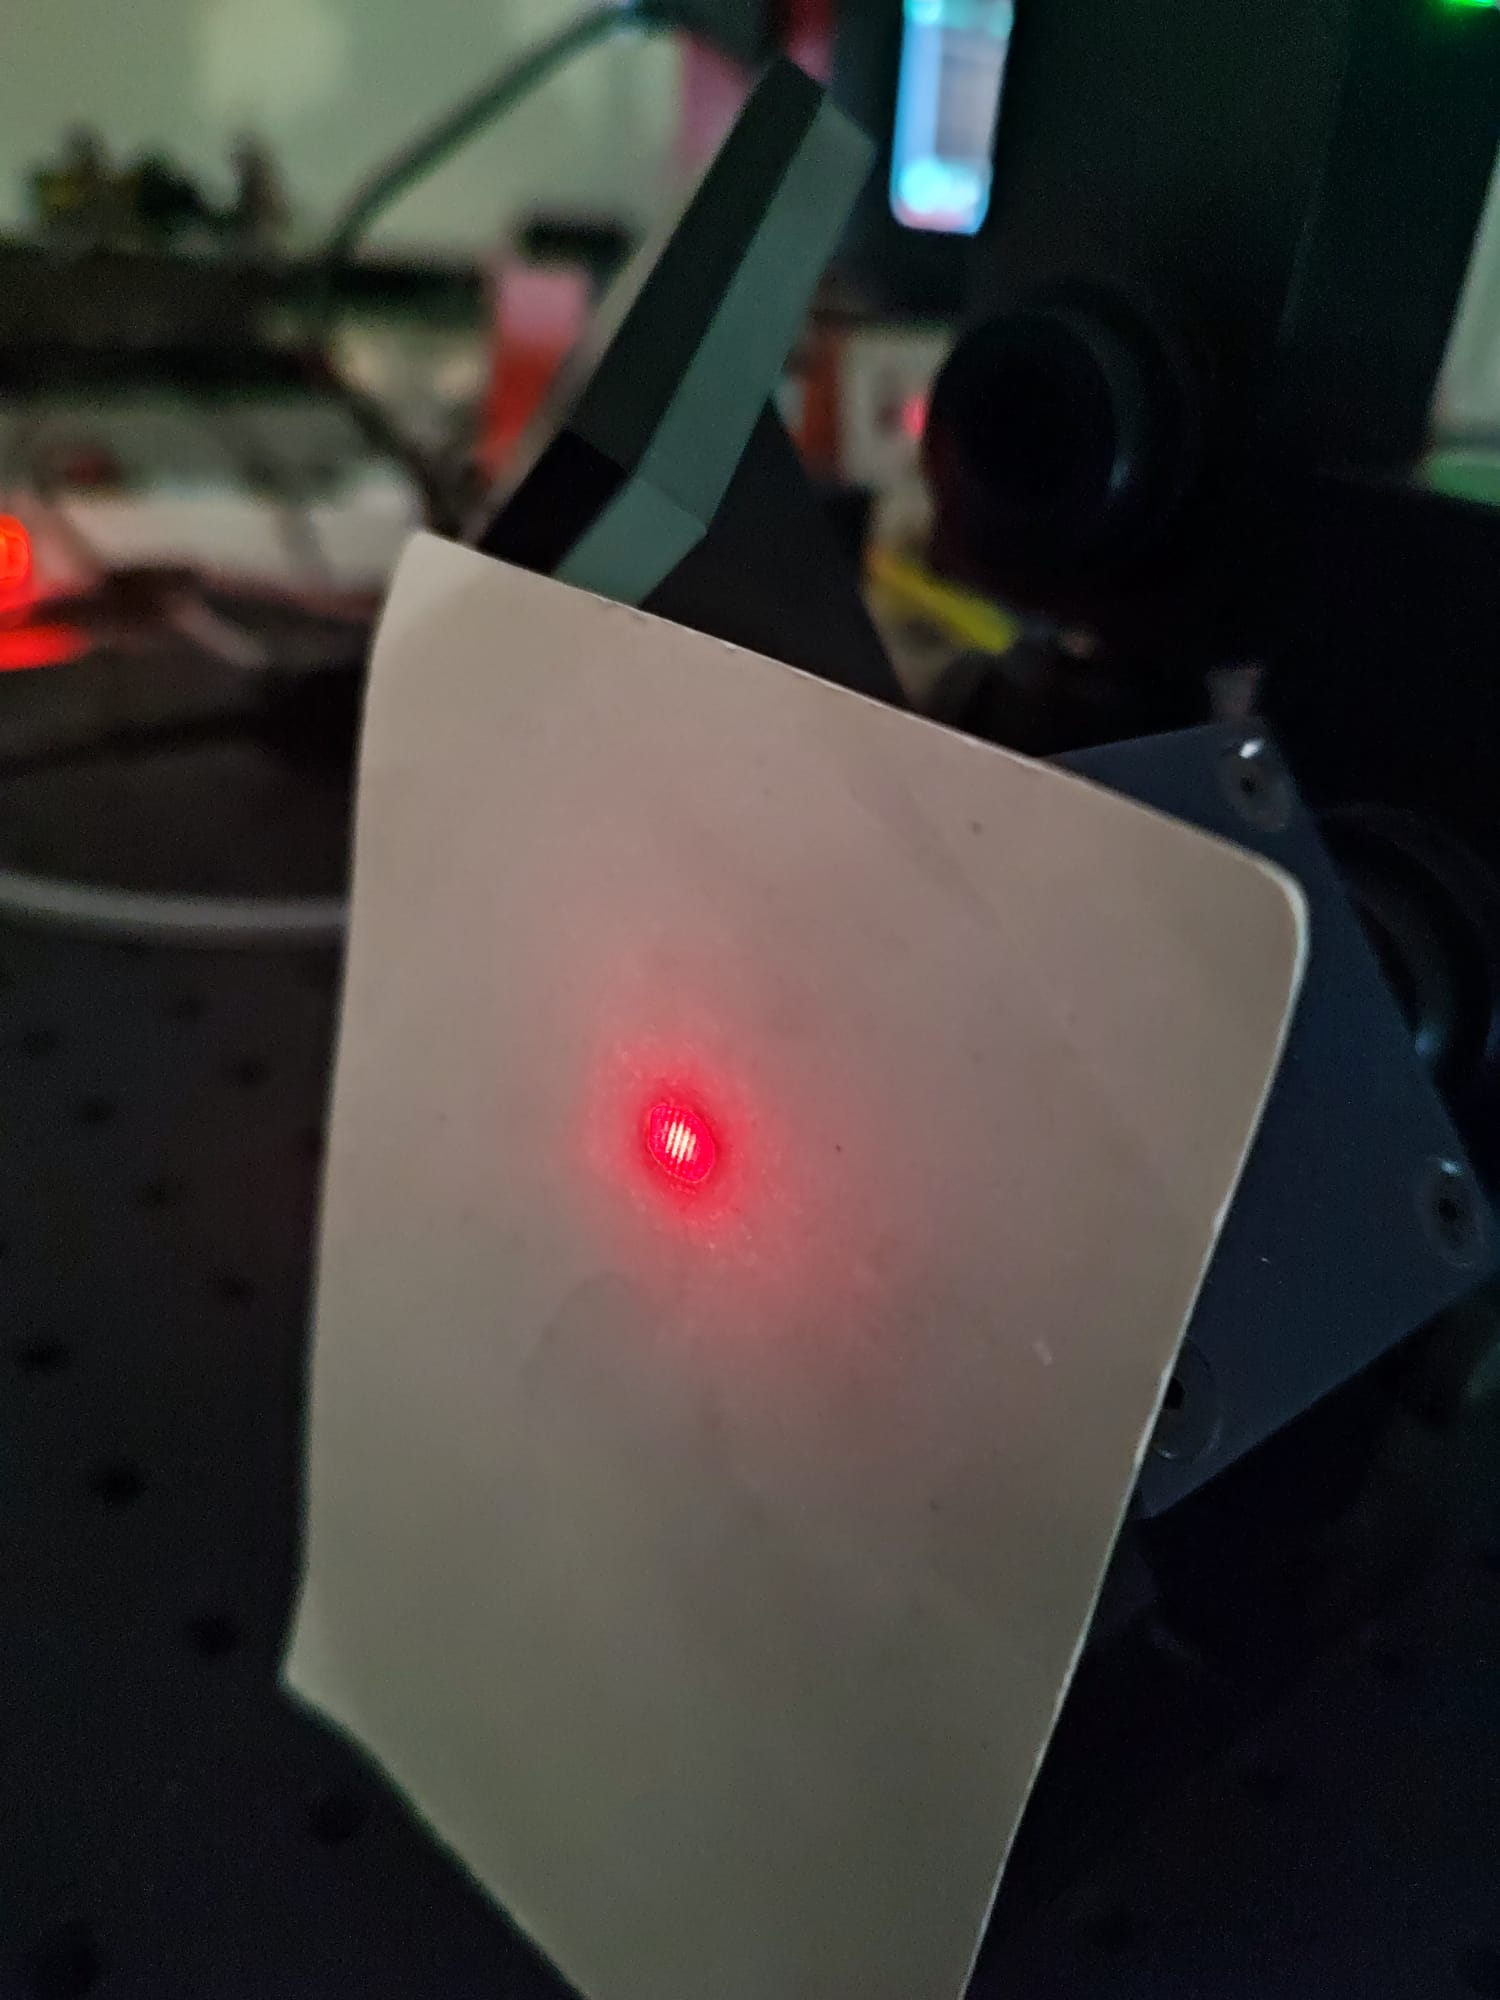
\includegraphics[width=2cm]{figures/streifen.jpeg}}
%    \subfigure[Ohne Streifen.]{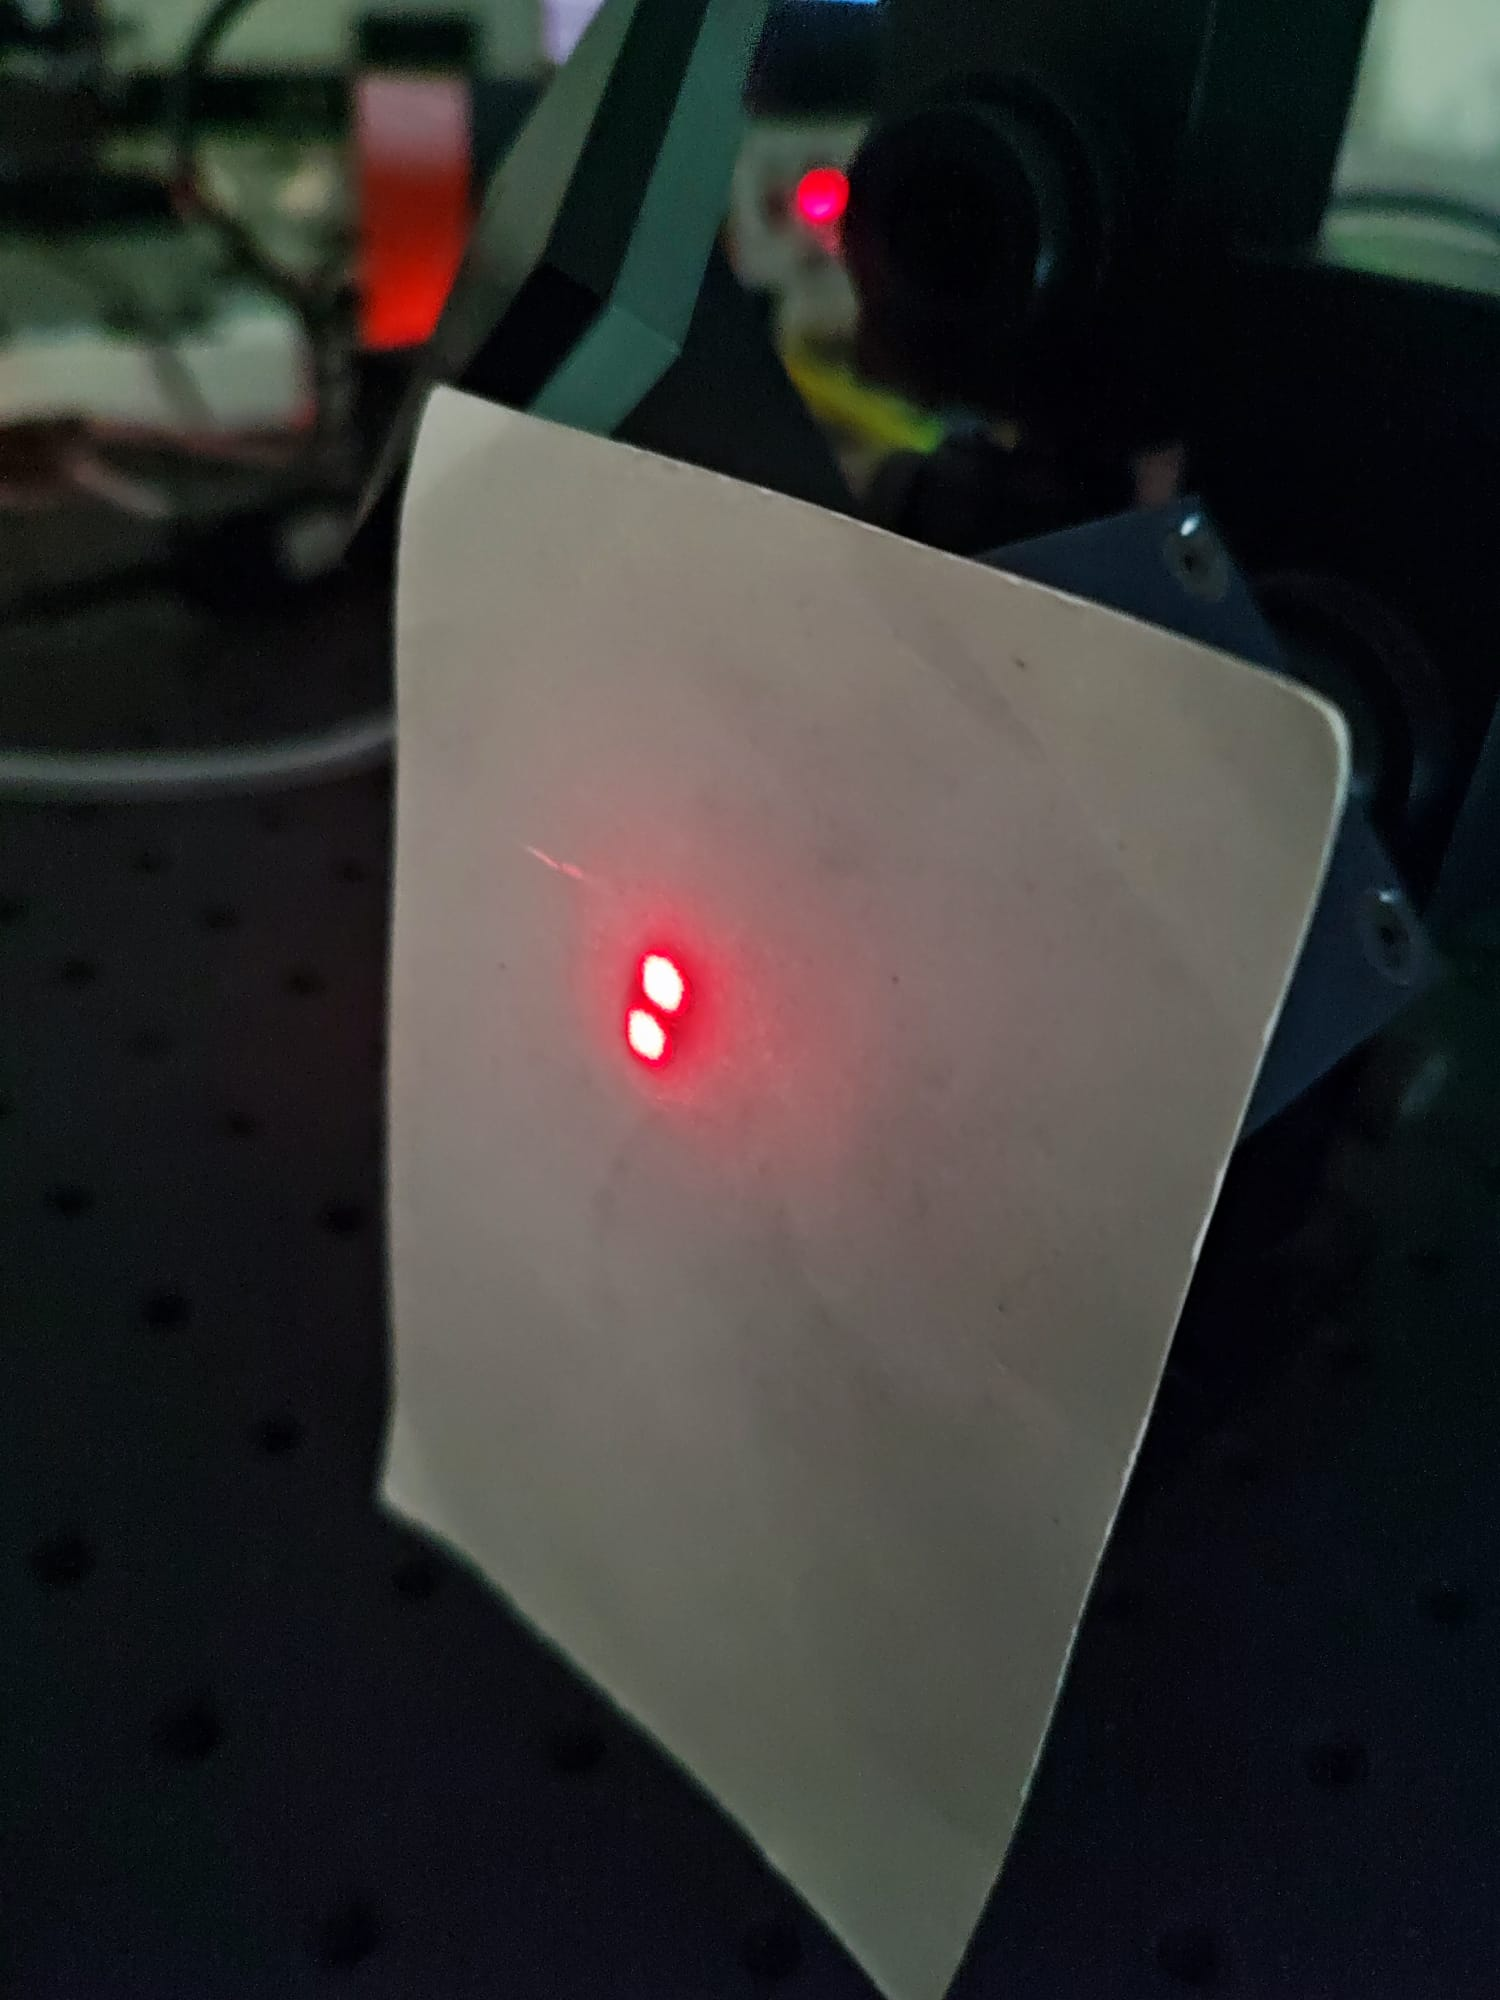
\includegraphics[width=2cm]{figures/ohnestreifen.jpeg}} %wann waren da zwei Punkte?
%    \caption{Interferenzmuster auf dem Schirm. Links noch mit Streifen, rechts nach weiterer Justierung.}
%    \label{fig:streifen}
%\end{figure}

Die Streifen entstehen dadurch, dass die Strahlen nicht perfekt ausgerichtet sind und unter einem Winkel auf den Schirm treffen. Die Spiegel werden nachjustiert, sodass die Streifen verschwinden und die Strahlen somit über die gesamte Länge parallel ausgerichtet sind.

Nun werden die überlappenden Strahlen in zwei horizontal zueinander versetzte Strahlen getrennt, indem Spiegel M2 bewegt wird und der transmittierte Strahl somit durch ein äußeres Loch der Justageplatte fällt. Die getrennten Strahlen fallen am Ende wieder zu einem Strahl zusammen. Auftretende Interferenzstreifen werden durch Nachjustierung entfernt.

In den Strahlengang werden zwei Glasplatten der Dicke $T = \SI{1}{\milli\meter}$ eingesetzt, die zueinander um $10 \degree$ verkippt sind. Diese werden in einen Rotationshalter eingebaut, sodass sie gedreht werden können. Die Platten werden jeweils von einem der beiden Strahlen getroffen.

Der hinter dem Interferometer platzierte Polarisationsfilter wird entfernt und der Strahl trifft stattdessen auf einen zweiten PBSC, der die Polarisation erneut trennt und auf zwei Dioden projiziert. %noch was?

Auf das Interferometer wird schließlich eine Haube gesetzt, damit Luftschwankungen den Versuch nicht beeinflussen.

\begin{figure}
    \centering
    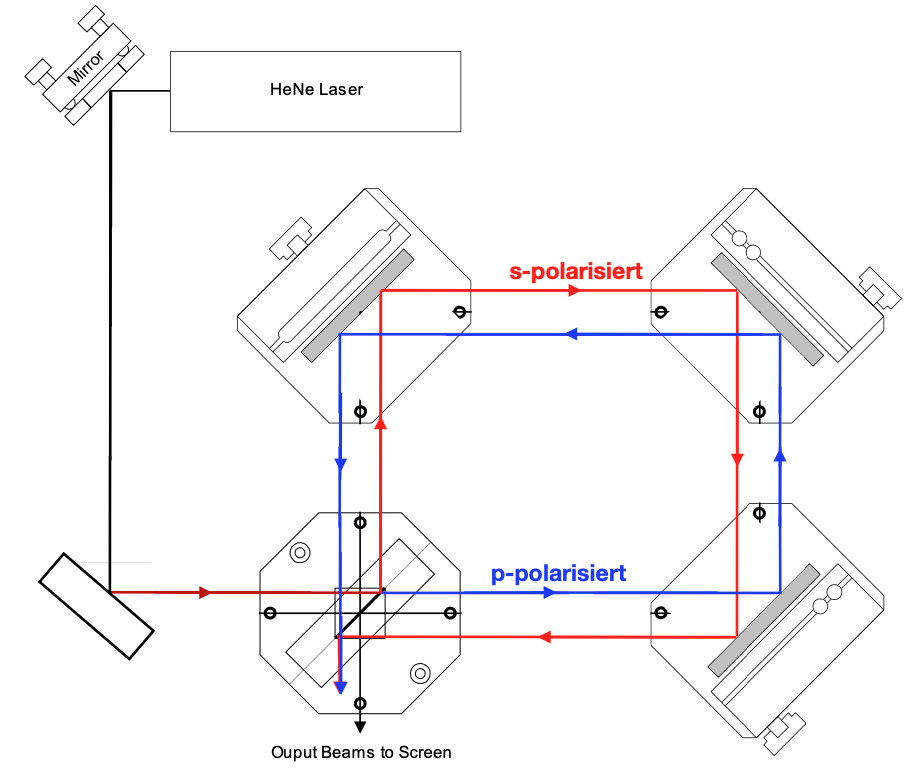
\includegraphics[width=0.7\linewidth]{figures/aufbau2.png}
    \caption{Der Strahlengang im Interferometer nach Aufteilen der beiden Strahlen. Der transmittierte Strahl ist in blau dargestellt, der reflektierte in rot. \cite{irgendeineseite}} %Quelle???
    \label{fig:strahlengang}
\end{figure}

\subsection{Messung}
\textbf{Kontrast des Interferometers}

Um den Kontrast des Interferometers zu bestimmen, wird der Winkel des Polarisationsfilters zwischen $0 \degree$ und $180 \degree$ in $15 \degree$-Schritten variiert und dabei jeweils die Diodenspannung des Interferenzmaximums und des Interferenzminimums aufgenommen. Die Maxima und Minima werden durch Drehung der Glasplatten gefunden.

Anschließend wird der Polarisationsfilter auf den Winkel eingestellt, bei dem der Kontrast am höchsten, also die Qualität des Interferometers am besten, ist. Hier beträgt dieser Winkel $\phi = 130 \degree$.
\\


\textbf{Brechungsindex von Glas}

Der Brechungsindex des verwendeten Glases soll bestimmt werden.
Hierbei wird die Differenzspannungsmethode verwendet. Beide Dioden messen also die Spannung und die Differenz wird mit Hilfe eines Operationsverstärkers gebildet. %oder wie heißt das?
Die Anzahl der Nulldurchgänge entspricht der Anzahl der Interferenzmaxima und -minima. %oder?
Der Vorteil dieser Methode ist es, dass mögliches Rauschen gefiltert wird, die Steigung um den Nulldurchgang größer ist und \dots %was noch?

Der Glashalter wird gedreht, während die Anzahl der Nulldurchgänge mit einem Zählwerk, auf das die Differenzspannung gegeben wird, gezählt wird. Die Messung wird zehn mal wiederholt.
\\


\textbf{Brechungsindex von Luft}

In diesem Teil des Versuchs wird ebenfalls die Differenzspannungsmethode verwendet.

Um den Brechungsindex von Luft zu bestimmen, wird eine Gaszelle mit einer Länge von $100 \pm 0.1 \si{\milli\meter}$ in den Strahlengang eingebaut. Ein Strahl läuft durch die Gaszelle, der andere verläuft frei. %umformulieren
Die Zelle wird zunächst evakuiert. Anschließend wird Luft wieder langsam eingeleitet und die Anzahl der Maxima und Minima wird in Abhängigkeit des Drucks gemessen. Dazu wird die Anzahl in $50 mbar$-Schritten abgelesen. Das Ganze wird drei mal wiederholt. %ging mit "\SI{50}{\milli\bar}" nicht?

Die Temperatur im Versuchsraum wird gemessen. Diese beträgt $\SI{19.4}{\celsius}$.



\section{Auswertung}
Im folgenden Abschnitt werden die erhaltenen Messwerte ausgewertet und die Ergebnisse diskutiert.
\subsection{Bestimmung des maximalen Kontrasts}
Um bei den eigentlichen Interferenzmessungen das bestmögliche Ergebnis zu erzielen ist die
Einstellung des optimalen Kontrasts notwendig.
Der Kontrast definiert als 
\begin{equation}
    K = \frac{U_\text{Max}-U_\text{Min}}{U_\text{Max}+U_\text{Min}}.
\end{equation}
Hierbei steht $U$ für die jeweilig gemessene Maximal- und Minimalspannung.
Um den größtmöglichen Kontrast zu bestimmten, wird der erste Polfilter über einen Bereich von 0 bis 180° 
variiert und mit Hilfe der drehbaren Schraube am Glasbehälter eine maximale und eine minimale Spannung am 
Multimeter eingestellt. 
Die aufgenommenen Messwerte und sich ergebenen Kontraste sind in \autoref{tab:Kontrast} dargestellt.
\input{build/tabKontrast.tex} 
\FloatBarrier
Mit Hilfe der Messwerte lässt sich eine Zusammenhang zwischen dem Kontrast und den Drehwinkel graphisch darstellen.
Dieser Plot ist in \autoref{fig:kontrast} dargestellt.
\begin{figure}
    \centering
    \includegraphics[width=0.7\linewidth]{build/Kontrast.pdf}
    \caption{Winkelabhängikeit des Kontrasts.}
    \label{fig:kontrast}
\end{figure}
\FloatBarrier
Der Kontrast hängt mit dem Polarisationswinkel $\theta$  über
\begin{equation}
    K(\theta) = \abs{ \alpha \sin{( \beta \theta
    + \gamma)}} + \delta
    \label{kontrast}
\end{equation}
zusammen. 
Die Fitparameter haben die Werte
\begin{align}
    \begin{split}
      \alpha &= \num{-0.89(6)}\\
      \beta  &= \num{2.008(29)}\\
      \gamma &= \SI{-0.18(5)}{\degree} \\
      \delta &= \num{0.020(30)}
    \end{split}
    \label{fitparameter}
\end{align}

\section{Bestimmung des Brechungsindexes von Glas}
Der Brechungsindex von Glas wird mit Hilfe der Differenzspannungsmethode bestimmt.
Dazu trifft der Laserstrahl auf einen um 45° gedrehten PBSC und anschließend in 2 Dioden.
In dem PBSC wird die Polarisatonsrichtung der überlappenden Laserstrahlen um 45° gedreht sodass
beide Laserstrahlen entweder p- oder s-polarisiert sind.
\footnote{Es spielt keine Rolle ob beide p-polarisiert oder beide s-polarisiert sind, die Hauptsache ist das sie eine 
einheitliche Polarisation aufweisen.}
Das detektierte Signal wird mit einer Operationsverärkerschaltung verarbeitet und auf einem
Oszilloskop abgebildet.
Mit der Differenzspannungsmethode ist es möglich ein wesentlich rauschärmeres Signal zu bekommen.

Der Brechungsindex lässt sich bestimmen indem der Rotationswinkel an der Stellschraube des Glasbehälters
über einen Bereich von 10° verändert wird und die dabei auftretenden Maxima/Nulldurchgänge am
Oszilloskop gezählt werden.
In \autoref{tab:Maxima} sind die Anzahlen der aufgetretenden Maxima dargestellt.
\input{build/tabMaxima_Glas.tex}
\FloatBarrier
Im Mittel sind demnach 34,7 Maxima aufgetreten.\\
Mit der Formel
\begin{equation}
    n = \left( 1 - \frac{\lambda{M}}{2T\theta_0\theta} \right)^{-1}
  \label{brech_glas}
\end{equation}
ergibt sich ein Brechungsindex von $1,566 \pm 0,021$.\\
Hierbei ist $T=\SI{1}{\milli\meter}$ die Dicke des Glases, $\lambda=\SI{632,990}{\nano\meter}$ die 
Wellenlänge des Lasers, $M$ die Anzahl der Maxima, $\theta_0$ der Verkippungswinkel der Gläser im Glashalter und
$\theta$ der Drehwinkel über einen Bereich von 10°.

%\begin{figure}
%    \centering
%    \includegraphics[width=0.7\linewidth]{./figures/xxx.xxx}
%    \caption{xxx}
%    \label{fig:xxx}
%\end{figure}
%
%\begin{equation}\label{eq:xxx}    
%    \begin{split}
%        \lambda &= \SI{855}{\angstrom}\\
%        \delta_\text{ps} &= 0,6\cdot 10^{-6}\\
%        \delta_\text{si}&= 6,8\cdot 10^{-6} \\
%        n_\text{luft} &= 1 \\
%        n_\text{ps} &= 1 - \delta_\text{ps} \\
%        n_\text{si} &= 1 - \delta_\text{ps} 
%    \end{split}
%\end{equation}
 
\nocite{*}
\printbibliography{}
\end{document}